\appendix

\begin{table}[t]
\section{Additional Ablation on \mimi Codec}
  \centering
  \caption{\textbf{Ablation study on hyper-parameters of the \mimi codec}. We evaluate semantic modeling by reporting the error rate on a phonetic ABX discriminability task. To evaluate reconstruction quality, we compute VisQOL and MOSNet. ``Quantization rate'' refers to applying quantization to the latent space only $50\%$ of the time during training (independently from quantizer dropout), as described in \hyperref[sec:mimi]{Section ~\ref{sec:mimi}}.}
  \label{tab:mimi_ablations_appendix}
  \footnotesize
  \resizebox{\textwidth}{!}{
  \begin{tabular}{ccccc|ccc}
    \toprule
    Quantization & Transformer & Transformer & WavLM & Split & \multirow{2}{*}{ABX ($\downarrow$)} & \multirow{2}{*}{VisQOL ($\uparrow$)} & \multirow{2}{*}{MOSNet ($\uparrow$)} \\
    Rate & in encoder & in decoder & distillation & quantizer &  &  &  \\
    \midrule
     \xmark & \xmark & \xmark & \xmark & \xmark & 31.3\% & 2.37 & 2.85 \\
     \xmark & \checkmark & \xmark & \xmark & \xmark & 31.4\% & 2.30 & 2.82 \\
     \xmark & \xmark & \checkmark & \xmark & \xmark & 27.5\% & 2.30 & 2.93 \\
     \xmark & \checkmark & \checkmark & \xmark & \xmark & 29.0\% & 2.25 & 2.94 \\
     \checkmark & \xmark & \xmark & \xmark & \xmark & 29.1\% & 2.65 & 2.86 \\
     \checkmark & \checkmark & \xmark & \xmark & \xmark & 27.4\% & 2.69 & 2.83 \\
     \checkmark & \xmark & \checkmark & \xmark & \xmark & 23.6\% & 2.72 & 2.89 \\
     \checkmark & \checkmark & \checkmark & \xmark & \xmark & 23.3\% & 2.82 & 2.89 \\
     \checkmark & \checkmark & \checkmark & \checkmark & \xmark & 6.5\% & 2.13 & 2.87 \\
     \checkmark & \xmark & \checkmark & \checkmark & \checkmark & 10.8\% & 2.68 & 2.84 \\
     \checkmark & \checkmark & \xmark & \checkmark & \checkmark & 8.1\% & 2.49 & 2.71 \\
     \xmark & \checkmark & \checkmark & \checkmark & \checkmark & 8.0\% & 2.36 & 2.88 \\
     \checkmark & \checkmark & \checkmark & \checkmark & \checkmark & 8.1\% & 2.72 & 2.89 \\
    \bottomrule
  \end{tabular}
  }
\end{table}

\section{Audio Matching and Deduplication}
\label{sec:audiomatching}

We have developed an audio matching system, whose objective is twofold:
\begin{enumerate}
\item \textit{Deduplication of source content}. Removing frequent duplicates to avoid overfitting and the regurgitation of audio content that is over-represented in the dataset, as evaluated in \hyperref[sec:regurgitation]{Section~\ref{sec:regurgitation}}.  \\[-1.7em]
\item \textit{Indexing solution}. By collecting signatures of samples at generation time, we can find if some content has been generated by our online demo or not by direct retrieval. 
\end{enumerate}

Our audio matching solution is inspired by the work of \cite{wang2003industrial}, as it offers a good trade-off between efficiency and effectiveness. This method is a retrieval system: Given a query, it detects the similar audio in a pre-indexed dataset. In our case, the signature design favors the de-duplication use-case, which needs to be more efficient: Formally, we need to compare every audio of the dataset with the whole dataset, which raises efficiency issues.  The signature extraction is described below. 


\paragraph{Constellation map.}
The first step to produce the signatures involves computing a set of keypoints referred to as a \emph{constellation map}. Our procedure is inspired by \cite{wang2003industrial} and  illustrated in \hyperref[fig:hash_extraction]{Figure~\ref{fig:hash_extraction}}. First, (1) we compute a mel-spectogram from the audio signal, where the time is discretized with frequency 40Hz and the frequency range into 64 bins. We then apply three filters to select time-frequency positions: (2) The energy filter ensures that we only select positions that are robust enough; (3) The time and (4) frequency filters ensure that we select maxima w.r.t. time and frequency. The combination of these filters is (5) a constellation, from which we extract hashes. 
\medskip

\begin{figure}[t]
\setlength{\parindent}{0cm}
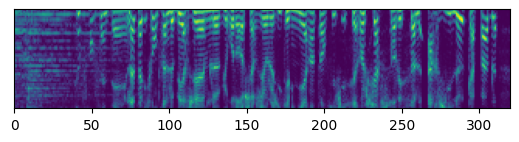
\includegraphics[width=0.48\linewidth,trim={0cm 0.84cm 0 0},clip]{figures/loreille/loreille_1.png}
\hfill
\raisebox{23pt}{\begin{minipage}[t]{0.5\linewidth}
(1) Mel-spectogram: The [200Hz--3000Hz] frequency range is split into 64 bands.  
\end{minipage}}

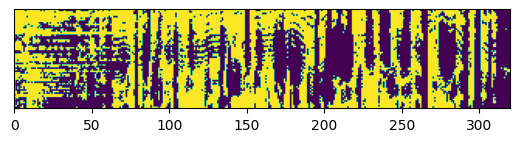
\includegraphics[width=0.48\linewidth,trim={0cm 0.84cm 0 0},clip]{figures/loreille/loreille_2.png}
\hfill
\raisebox{23pt}{\begin{minipage}[t]{0.5\linewidth}
(2) Energy filter: filter our all positions (time, band) whose amplitude is below the average.
\end{minipage}}

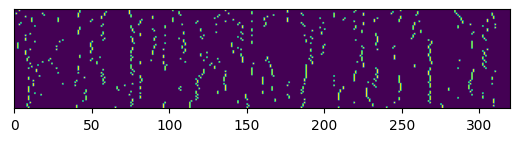
\includegraphics[width=0.48\linewidth,trim={0cm 0.84cm 0 0},clip]{figures/loreille/loreille_3.png}
\hfill
\raisebox{23pt}{\begin{minipage}[t]{0.5\linewidth}
(3) Time filter: keep only position with highest mel-spec value in a sliding window. 
\end{minipage}}

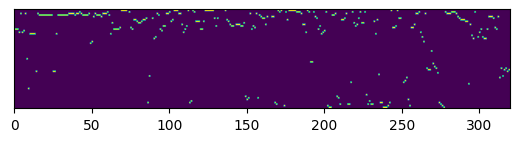
\includegraphics[width=0.48\linewidth,trim={0cm 0.84cm 0 0},clip]{figures/loreille/loreille_4.png}
\hfill
\raisebox{23pt}{\begin{minipage}[t]{0.5\linewidth}
(4) Frequency filter: At a given time, keep only the most energetic frequency band. 
\end{minipage}}

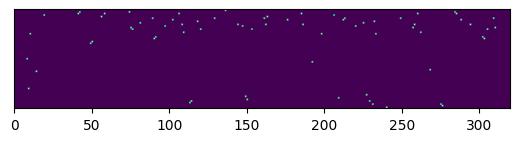
\includegraphics[width=0.48\linewidth,trim={0cm 0.84cm 0 0},clip]{figures/loreille/loreille_5.png}
\hfill
\raisebox{23pt}{\begin{minipage}[t]{0.5\linewidth}
(5) The Constellation map obtained by intersecting the three filters above. 
\end{minipage}}
\caption{\textbf{Mel-spectrum keypoint extraction}. Three filters are applied to the audio mel-spectrum to extract a constellation of keypoints on which hash signatures are computed.
\label{fig:hash_extraction}}
\end{figure}

At the end of the keypoint extraction procedure, the constellation map ${\mathcal C}$ consists of a list of $n$ tuples of the form ${\mathcal C}=\{(t_i, f_i)\}_{0 \leq i < n}$, where each selected timestamp $t_i$ is associated with a mel-spec discrete frequency level $f_i \in \{0,\dots,63\}$ . 

\paragraph{Hash encoding.} 
From the constellation map, we extract hash signatures as follows. For each keypoint $(t_k, f_k) \in \mathcal C$, we select, if there exists:
\begin{itemize}
\item A forward keypoint $(t_\mathrm{f},f_\mathrm{f})$, which is the closest time to $t_k$ such that $t_k+m \leq t_\mathrm{f} < t_k+M$, where $[t_k+m,t_k+M)$ is the temporal window from which we select a keypoint. Note, for a given $t_\mathrm{f}$, the corresponding frequency $f_\mathrm{f}$ is unique by design of the filters. 
\item A backward keypoint $(t_\mathrm{b},f_\mathrm{b})$, which is determined by the keypoint closest in time to $t_k$ such that $t_k-M < t_\mathrm{b} \leq t_i-m$, where $(t_k-M,t_k-m]$ is the temporal window in which the procedure selects a keypoint. 
\end{itemize}

We extract a signature only if both the forward and backward keypoints exist. In that case the signature is defined by the tuple $s_k=(f_\mathrm{b},f_k,f_\mathrm{f},t_k-t_\mathrm{b},t_\mathrm{f}-t_k)$, which we associate to the absolute timestamp $t_k$. 
In our case we set $m=4$ and $M=20$. Therefore the maximum time-span of the signature is $2\cdot M$, i.e., about 3.2 seconds. 
Formally, the hash key can take $64^3 (M-m)^2 = 2^{26} = 67,108,864$ distinct values. In practice the distribution of hash values is skewed and some signatures are unlikely to occur. 
 

\paragraph{Pair-wise matching and one-to-many comparison.} With our signature extraction, we can compare two audios by comparing their signature sets, which amounts to computing the intersection of the hash-keys. When one wants to compare a query audio to a dataset that consists of many audios, it is more efficient to perform this comparison with an inverted file or a hash table. In that case, the indexing structure returns the lists of matching signatures along with the matching timestamps for each of the audio. Similar to \cite{wang2003industrial}, we only preserve the matches that are temporally consistent thanks to a simple Hough 1D temporal voting scheme. Optionally, we incorporate a tolerance of $\pm 1$ on the timestamps $t_\mathrm{b}$ and $t_\mathrm{f}$ when matching the signatures. This tolerance increases the complexity and we therefore do not use it for the dataset deduplication case. 

\paragraph{De-duplication: Signature fused set.} 
For our deduplication strategy, we first cross-match all the audio segments in the dataset, and extract the matching segments that occur often enough (typically $\geq 10$ matches). Since their signatures are redundant, we remove all duplicate signatures that occur at identical relative timestamps to produce a single \emph{duplicate signature set}. At training time, in order to determine if an audio segment is a frequent duplicate to be filtered out, we simply compare its signature set to the duplicate signature set. In other terms, we simply perform  a simple audio-to-audio matching between the putative training segment and the synthesized duplicate signature file. We use the segment for training only if the score is below a pre-defined matching threshold. 


\section{Delayed text LM as a zero-shot streaming ASR and TTS}
\label{app:streaming_tts}
As explained in \hyperref[sec:interleaving]{Section~\ref{sec:interleaving}}, Moshi models audio tokens, along
with a text stream that is aligned on the audio frame rate with the use of special padding tokens, as represented in \hyperref[fig:rainbow]{Figure~\ref{fig:rainbow}}. We can adapt this method for ASR and TTS by introducing a delay between the audio and text tokens. In both cases, the model operates in full streaming mode, with a fixed latency (here 2 seconds).
    
\paragraph{ASR mode.} If the audio is ahead of the text, we ignore the model prediction for the audio tokens, using instead those of some audio input, and sample the text tokens freely. Then the text stream contains the audio transcription, with fine alignments at the word level, as depicted in \hyperref[fig:rainbow_asr]{Figure~\ref{fig:rainbow_asr}}.
\paragraph{TTS mode.} If the text is ahead of the audio, we can symmetrically derive a TTS engine. We need for that a properly padded set of text tokens. We obtain those in a zero-shot manner by allowing the model to sample freely \texttt{PAD} and \texttt{EPAD} tokens. As soon as the model tries to sample a different token, we instead input the next word to generate. Note that we can further control the rate of the speech by keeping an online average of the fraction of padding tokens. By introducing a small bonus on their logits when this fraction falls below a given target value, we ensure reasonable rate and a good intelligibility in all situations. Finally, using a prefix with both text and audio tokens, we can control the voice of the speaker. A representation is given in \hyperref[fig:rainbow_tts]{Figure~\ref{fig:rainbow_tts}}.
\paragraph{Multi-stream TTS.} We use this mechanism both in single and multi-stream mode. In multi-stream mode, the model outputs two sets of audio tokens. The text is provided in a single stream, using the \texttt{<bos>} and \texttt{<eos>} tokens to separate the text from the two speakers.


\begin{figure}
\centering
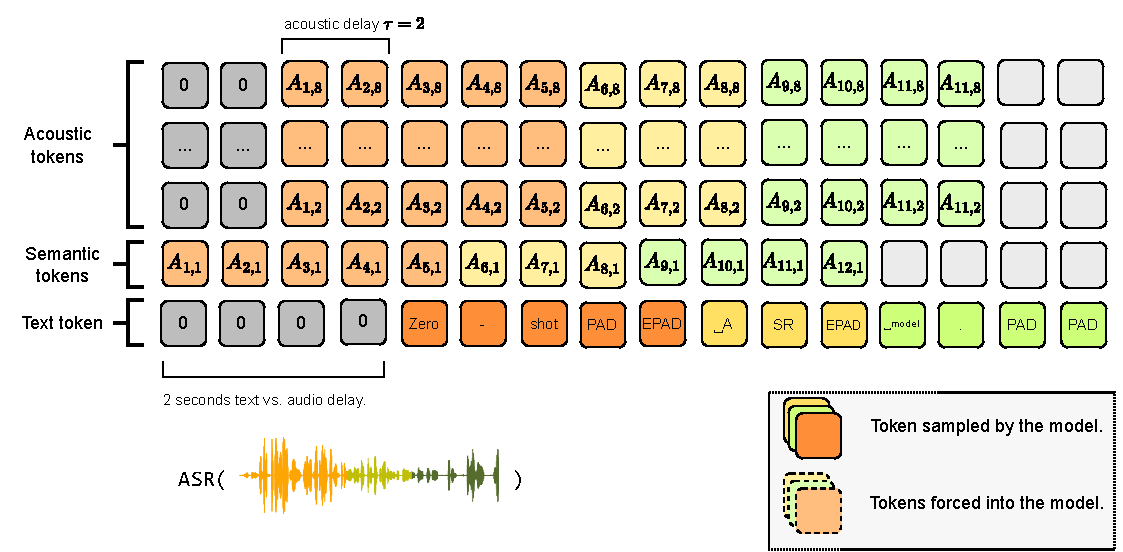
\includegraphics[width=\textwidth]{figures/ASR.drawio.pdf}
\caption{\textbf{Representation of the joint sequence modeled by Moshi when used for ASR.}
Each column represents the tokens for a given step in the joint sequence $(V_{s, k})$, similar to the one described in \autoref{eq:final_multi_sequence}, but adapted for ASR. The text is delayed by 2 seconds, and we use an acoustic token delay $\tau=2$. Tokens are predicted from bottom to top in the depth Transformer.
The audio tokens are kept to match those of the input audio, while text tokens are sampled freely. This also provides fine word timestamps.}
\label{fig:rainbow_asr}
\end{figure}


\begin{figure}
\centering
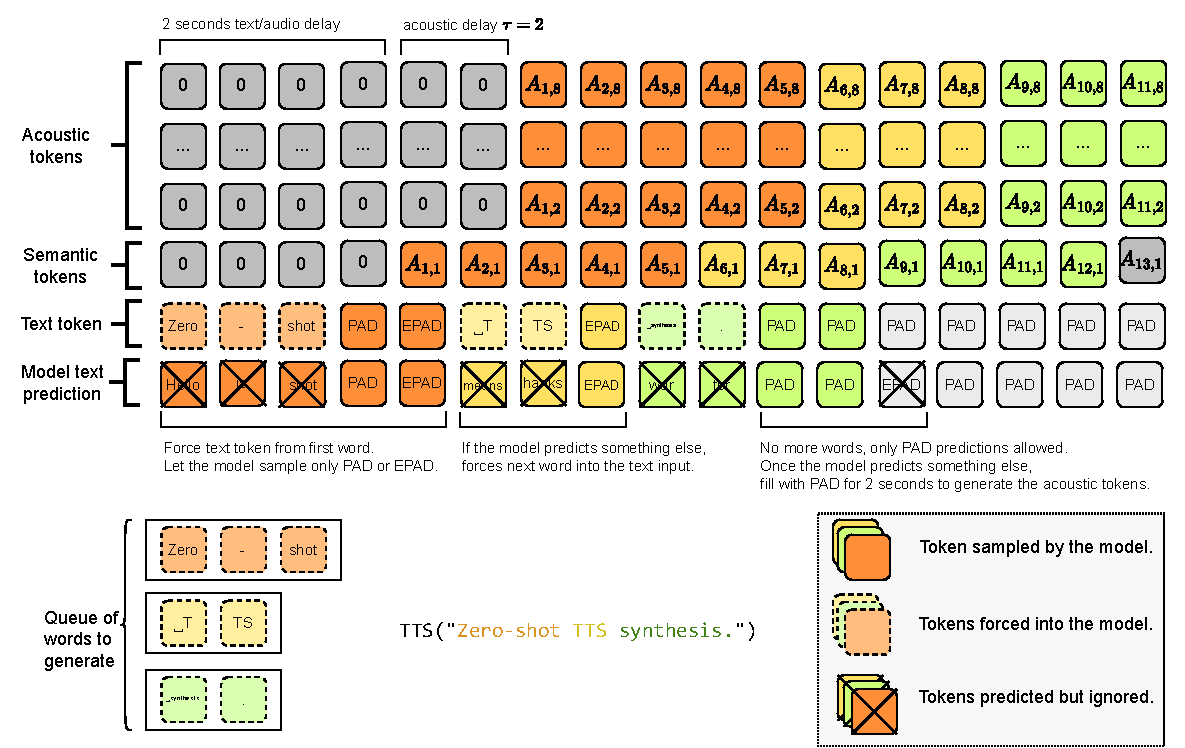
\includegraphics[width=\textwidth]{figures/TTS.drawio.pdf}
\caption{\textbf{Representation of the joint sequence modeled by Moshi when used in TTS mode}. Each column represents the tokens for a given step in the joint sequence $(V_{s, k})$, similar to the one described in \autoref{eq:final_multi_sequence}, but adapted for TTS. The audio is delayed by 2 seconds, and we use an acoustic token delay $\tau=2$. Tokens are predicted from bottom to top in the depth Transformer.
Text predictions are usually ignored, and the tokens from the text to generate are used instead. However,
this text input lacks padding token. At the end of each word, we allow the model to sample freely \texttt{PAD} and \texttt{EPAD} tokens. If the model tries to sample another token, we instead use the tokens from the next word. The semantic and acoustic audio tokens are sampled normally, being implicitly conditioned on the text due to the delay used. This method also provides a fine alignment of the words in the generated audio, by noting the time at which a given word is consumed by the model.
}
\label{fig:rainbow_tts}
\end{figure}




\newpage
\section{Characterizing Audio Artifacts Caused by Quantization}
\label{app:artifactsmetric}

First, recall that Moshi jointly handles three streams of tokens, text tokens $W_{s}$ for Inner Monologue, semantic+acoustic audio tokens $(A_{s, k})_{1 \leq k \leq Q}$ for Moshi's audio, and the similar audio tokens $(A'_{s, k})_{1 \leq k \leq Q}$ for the user's input. 
To analyse the impact of model quantization on genereated content, we first compute the Shannon entropy $H$ across windows of fixed size $C$ at each timestep $s$ for the 
text and Moshi's audio streams independently. This yields $H^{0}_s = H(W_{s-C:s})$ for text, and $H^{k}_s = H(A_{s-C:s, k})$ for each audio level. 
We use  $C = 64$ in practice, which corresponds to roughly 4.5 seconds of audio once decoded, and ignore all the leading $C$ tokens as they have a reduced context (furthermore, in our experimental scenario, they include the initial  prompt used for generation).

We observe qualitatively that the entropy spectrum is often indicative of artifacts or degradations of the audio samples. 
Formally we define three types of  artifacts from the entropy statistics, as described below. In practice, we characterize the presence or absence of each artifact over non-overlapping windows of  $\omega = 64$ tokens, as illustrated in \hyperref[fig:artifactsexampleextended]{Figure \ref{fig:artifactsexampleextended}}. 
\looseness=-1
\paragraph{Repetitive text.}
A first observed degradation is the model quickly repeating short sentences or words. This is characterized by the text entropy being almost flat over a window $H^0_{s:s+\omega}$, but non zero (as more than one token is repeated), as seen in  \hyperref[fig:artifactsexampleextended]{Figure \ref{fig:artifactsexampleextended}\,(c)}. We measure the ``flatness" of $H^0_{s:s+\omega}$ by fitting a linear regression model to it and verifying whether the slope is below a certain threshold hyper-parameter $\eta_\text{flat} = 10^{-3}$.
\looseness=-1
\paragraph{Silence vs. background noise.} 
By design, Moshi being silent corresponds to a constant stream of \texttt{PAD} text tokens (hence $H^0_{s:s+\omega} = 0$), while simultaneously, the corresponding audio tokens decode to a near silent waveform: The audio tokens are not constant, but fall into a small subset of ``silence tokens", which results in a  lower overall entropy for the audio tokens as seen for instance in the short silences of \hyperref[fig:artifactsexampleextended]{Figure \ref{fig:artifactsexampleextended}\,(a)}. We measure this behavior as  $\text{median}_{k > 1, s}(H^k_{s:s+\omega}) \leq \eta_{\text{audio\_silence}} = 2 $.
Note that \textit{we do not consider these silences to be artifacts}: This is because silences occur naturally in the multi-stream model as they simply represent the other speaker's turn. For illustration purposes, we highlight silences throughout \hyperref[fig:artifactsexampleextended]{Figures \ref{fig:artifactsexample} and \ref{fig:artifactsexampleextended}}, but we  count them as artifact-free timesteps otherwise.

In contrast, \emph{background noise} artifacts occur when the text stream is silent ($H^0_{s:s+\omega} = 0$), but audio tokens still have a rich output  ($\text{median}_{k > 1, s}(H^k_{s:s+\omega}) > \eta_{\text{audio\_silence}} $). This is shown in \hyperref[fig:artifactsexampleextended]{Figure \ref{fig:artifactsexampleextended}\,(d)} where a silence slowly degrades into background noise over time. 
\looseness=-1
\paragraph{Bad audio quality.} The last category of artifacts encompasses degraded audio quality while the main speaker (Moshi) is speaking: 
\begin{itemize}
\item \emph{Gibberish} is a very common type of artifacts at low bitwidth quantization (W2) and corresponds to incoherent speech. It is easily characterized by a high entropy of the text token ($H^0_{s:s+\omega} > \eta_{\text{gibberish}} = 3.5 $), as shown in \hyperref[fig:artifactsexample]{Figure \ref{fig:artifactsexample}\,(b)}.

\item \emph{Noisy Audio} is harder to detect, as illustrated in \hyperref[fig:artifactsexampleextended]{Figure \ref{fig:artifactsexampleextended}\,(b)} for instance.
We characterize it by first assessing that we are not in either a silence or background noise case, and then testing whether the standard deviation of the tokens' entropy across the audio codebooks is above a certain threshold $\eta_\text{noise} = 0.6$. 
\end{itemize}

\begin{figure}[tbh]
\centering
\begin{minipage}[b]{0.45\textwidth}
\scriptsize
    \textbf{(a)} Example entropy spectrum of a good audio samples (no artifacts detected). Short pauses occur for the main speaker due to the multi-stream design.\\[-0.09cm]
   
    \centering
    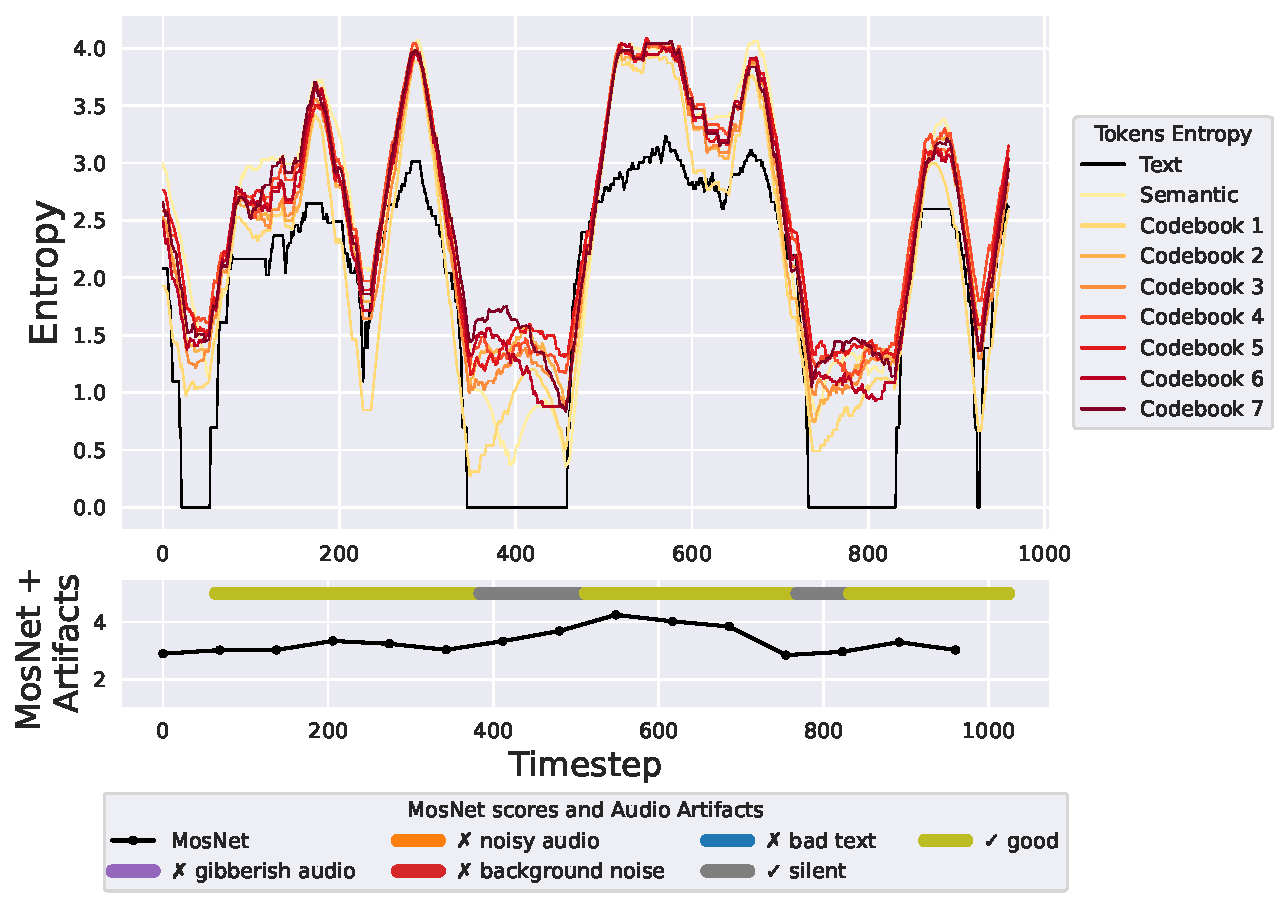
\includegraphics[width=\linewidth]{figures/quantized_models_mosnet/quant_artifacts_examples/good_sample_1.pdf}

\end{minipage}
~~~~
\begin{minipage}[b]{0.45\textwidth}
\scriptsize
    \textbf{(b)} Generally, the presence of artifacts tend to increase over time, here with repetition starting to occur in the speech.\smallskip
    
    \centering
    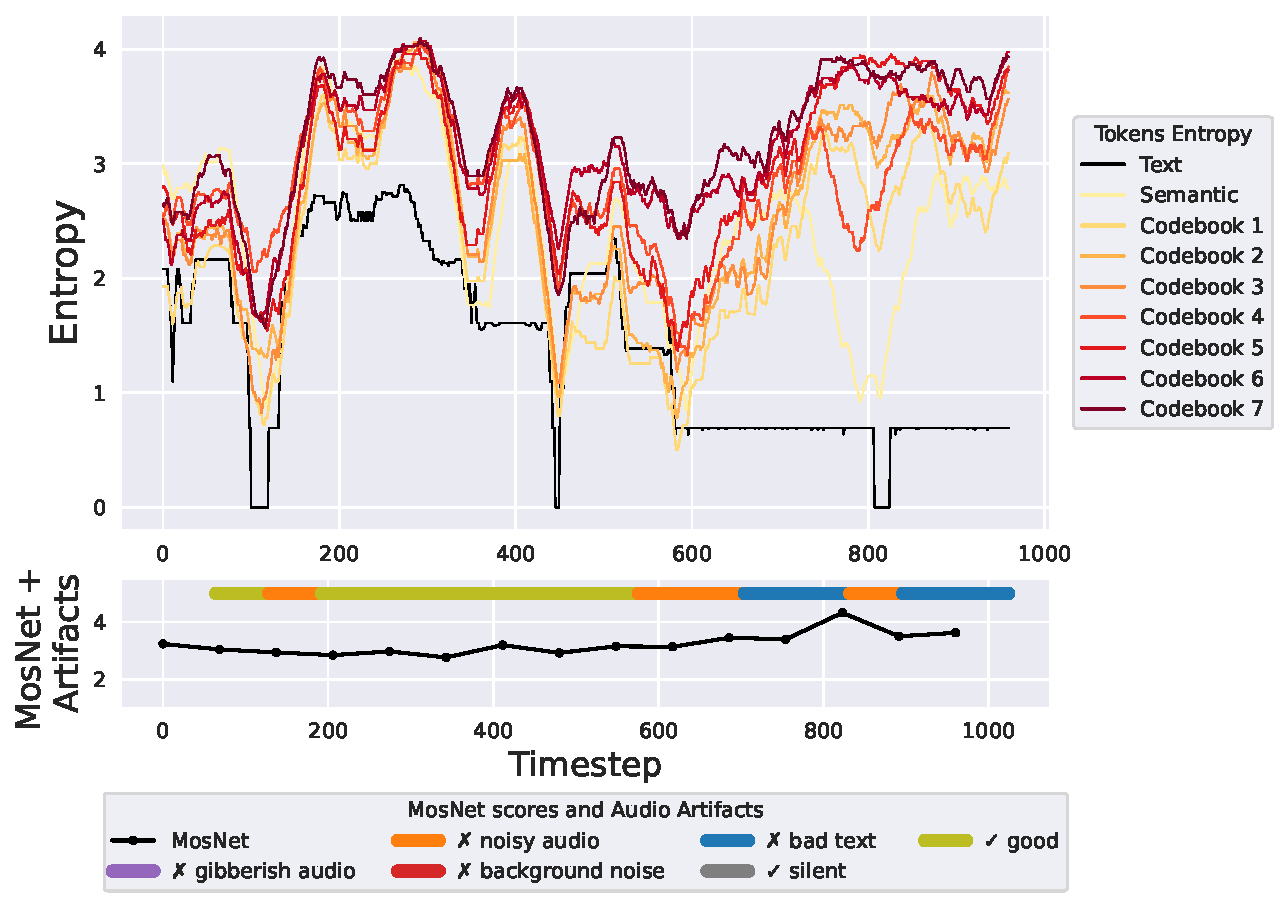
\includegraphics[width=\linewidth]{figures/quantized_models_mosnet/quant_artifacts_examples/repetitive_text_at_the_end.pdf}
\end{minipage}


\begin{minipage}[b]{0.45\textwidth}
\scriptsize
    \textbf{(c)} Another common artifact is repetitive snippets of text (with good audio quality), which are characterized by a flat entropy of the text token.\\[-0.09cm]
   
    \centering
    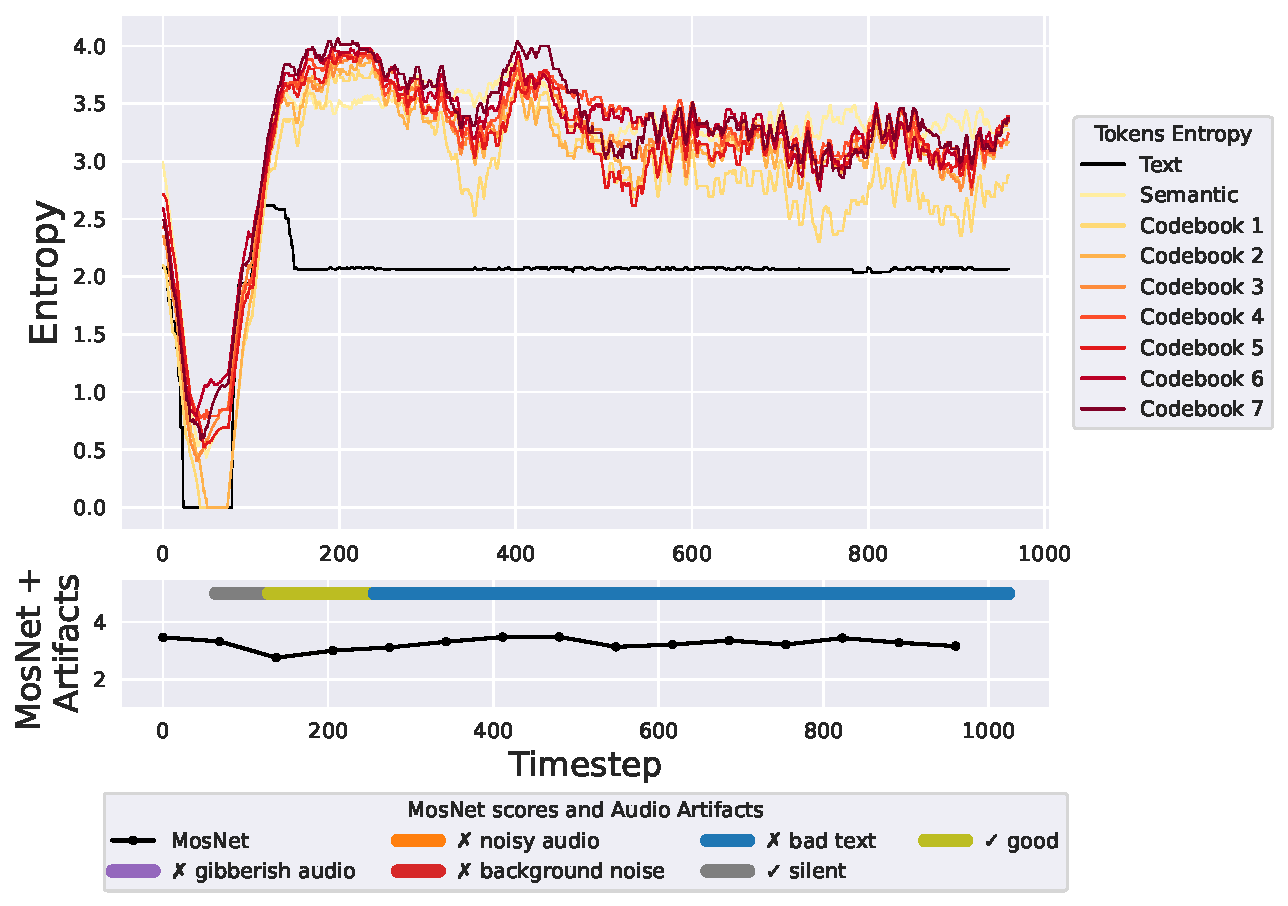
\includegraphics[width=\linewidth]{figures/quantized_models_mosnet/quant_artifacts_examples/repetitive_text.pdf}

\end{minipage}
~~~~
\begin{minipage}[b]{0.45\textwidth}
\scriptsize
    \textbf{(d)}Silences can degrade to background noise.\smallskip
    
    \centering
    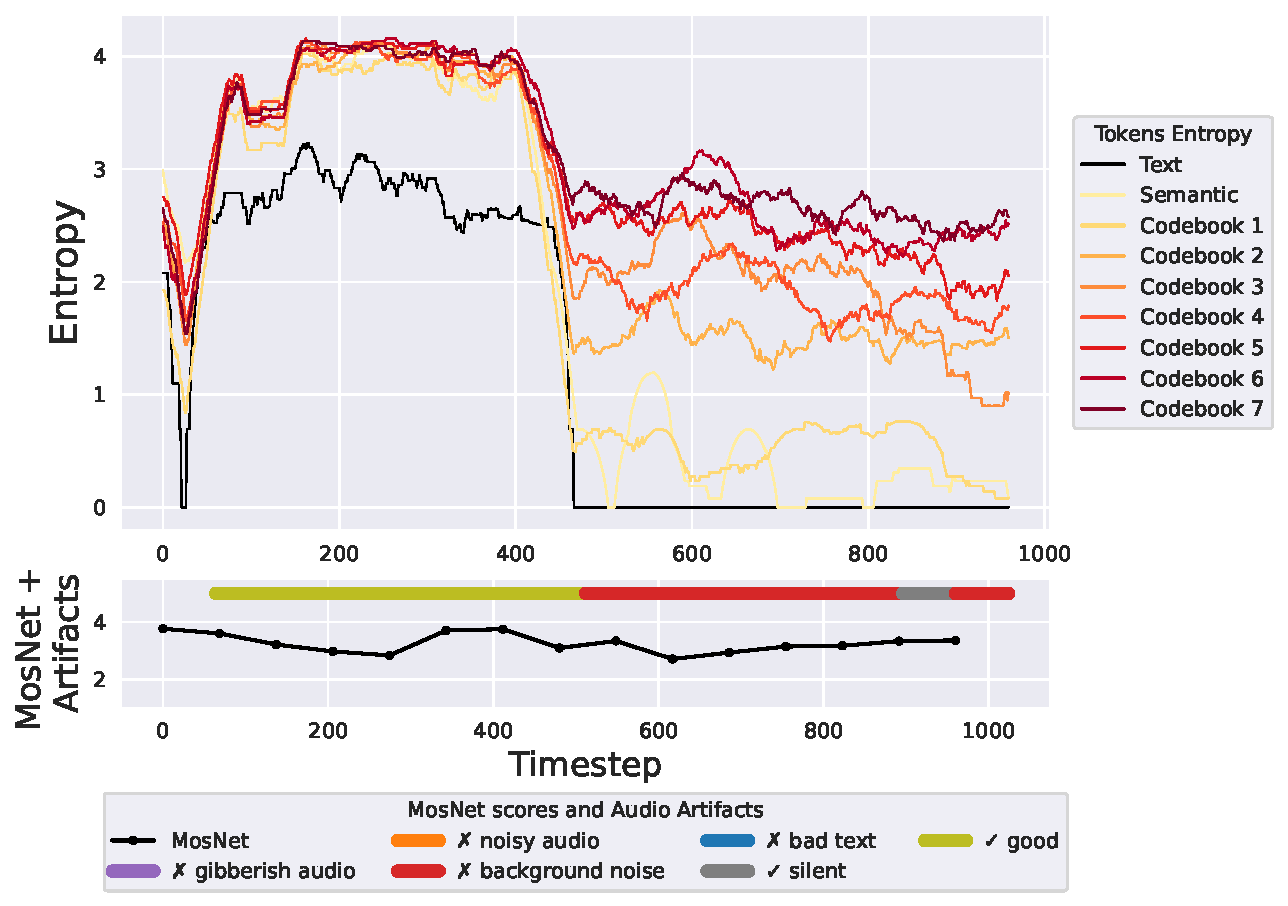
\includegraphics[width=\linewidth]{figures/quantized_models_mosnet/quant_artifacts_examples/silence_into_background_noise.pdf}
\end{minipage}

\caption{\label{fig:artifactsexampleextended}\textbf{Example of typical entropy spectrums capturing specific audio artifacts caused by model quantization}. For each timestep, we compute the entropy over the past 128 tokens, independently for the text and audio codebooks tokens. Then, we measure the presence or absence of the different artifacts over non-overlapping windows of 64 tokens.
    }
\end{figure}

While measuring the presence of these artifacts relies on several hyper-parameters, the thresholds $\eta_\text{flat}, \eta_{\text{audio\_silence}}, \eta_{\text{gibberish}}$ and $\eta_{\text{noise}}$  characterize the entropy of the sampled output tokens directly, thus are primarily related to the text/audio vocabulary, rather than the  weights of the Temporal and Depth Transformers. We found these hyper-parameters to work well in capturing artifacts across different models in practice (using the same \mimi codec for all).
Note that the values chosen for these hyper-parameters are also tightly linked with the chosen context size $C$ and window $\omega$, thus they are not particularly robust to changes on the temporal axis. In addition, choosing a too small value for $\omega$ may lead to false negative cases, e.g. by missing very short artifacts.
Nevertheless, as shown in \hyperref[fig:artifactsexampleextended]{Figure \ref{fig:artifactsexampleextended}}, this simple analysis of  the entropy spectrum offers additional fine-grained insights on the types of audio artifacts caused by model quantization, complementing the MOSNet scores obtained for the same samples.


Finally, in \hyperref[fig:artifacts]{Figure \ref{fig:artifacts}} we report the distribution of artifacts over time, averaged across 500 samples for each model: At a bitwidth of 4, there is still little difference in behavior between the unquantized model and the quantized ones. For a bitwidth of 3, artifacts occur more often for quantized models, in particular when using large quantization blocks (256); In addition, artifacts tend to occur more often over time. Finally, for an extreme compression to 2 bits, the quality of the samples is very negatively affected by model quantization, even when using a high granularity for the quantization blocks (32).


\begin{figure}%
    \centering
    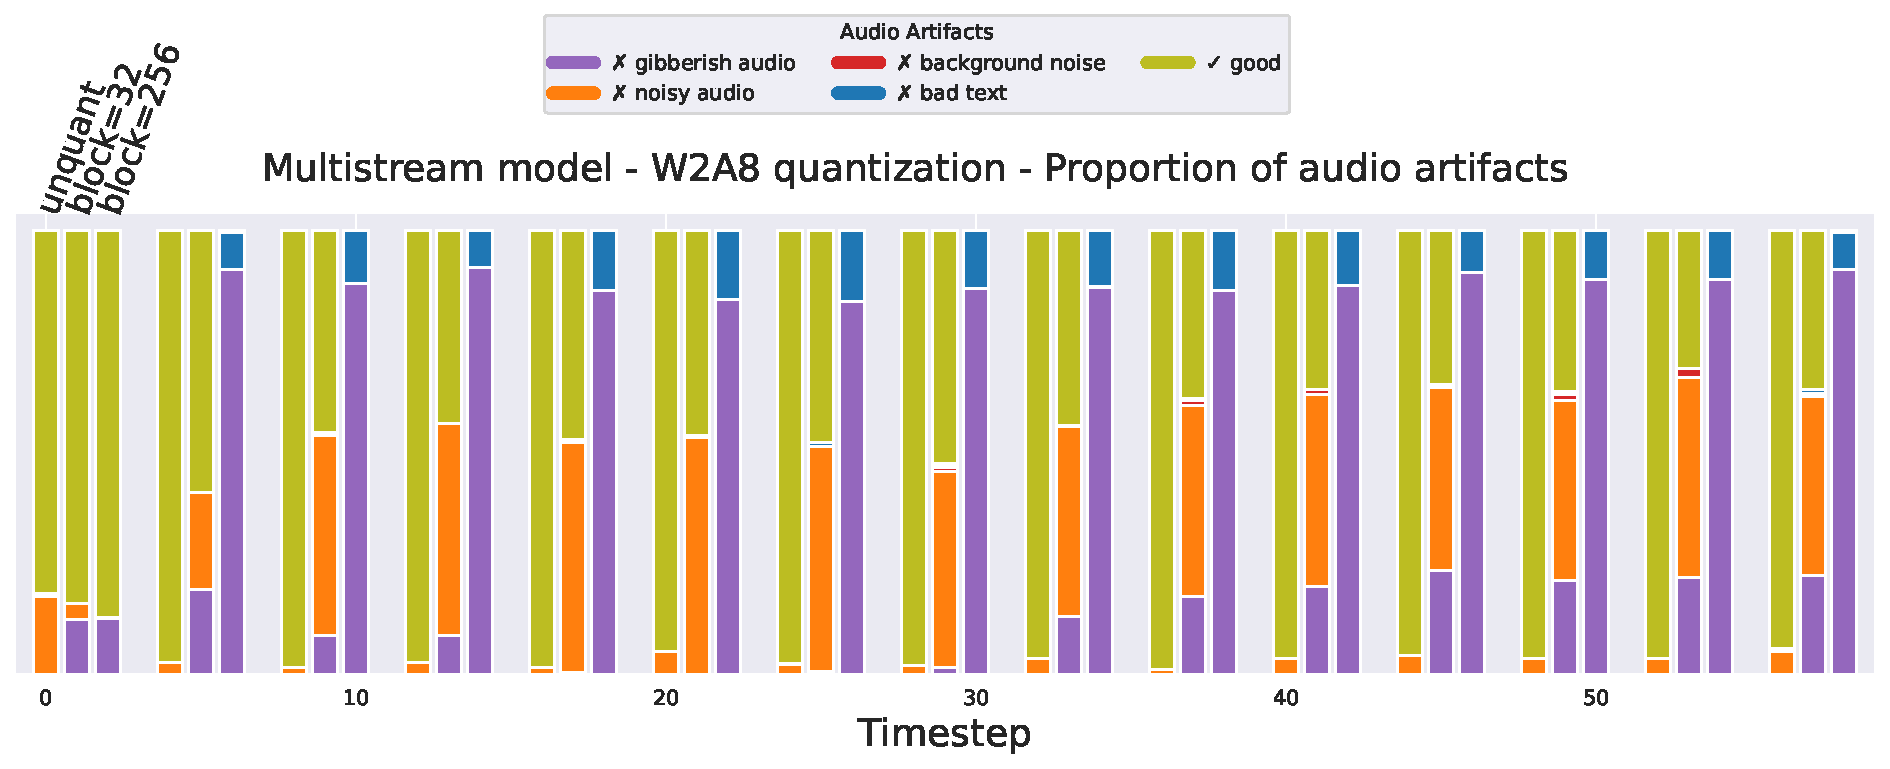
\includegraphics[width=0.95\textwidth]{figures/quantized_models_mosnet/quant_artifacts_summary_plots/8cf6db67_bs2_artifacts.pdf}
    
    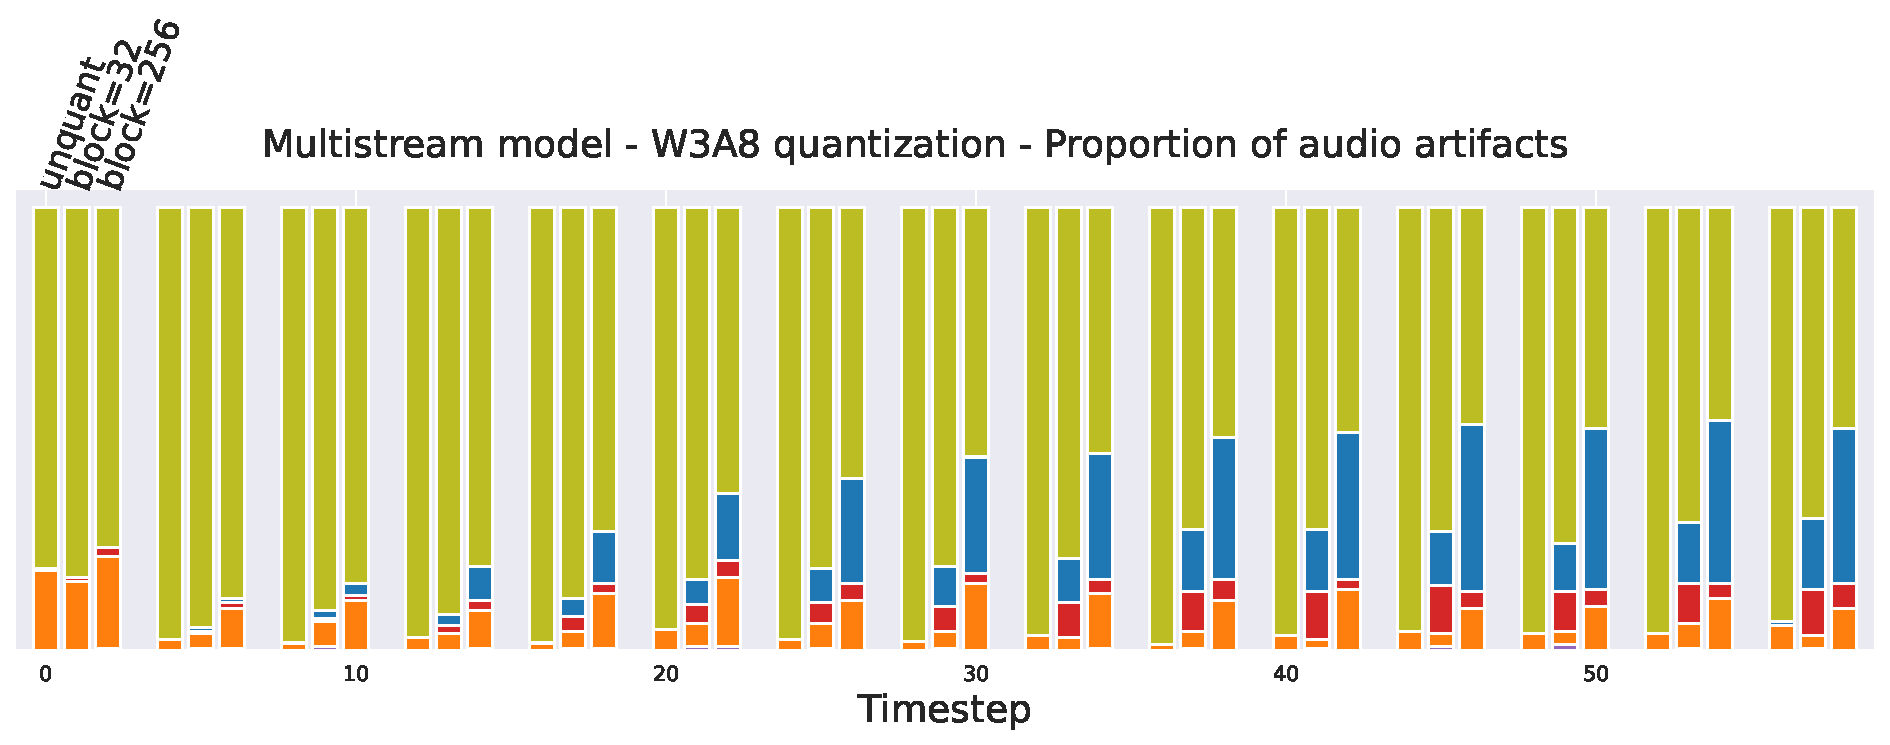
\includegraphics[width=0.95\textwidth]{figures/quantized_models_mosnet/quant_artifacts_summary_plots/8cf6db67_bs3_artifacts.pdf}
    
    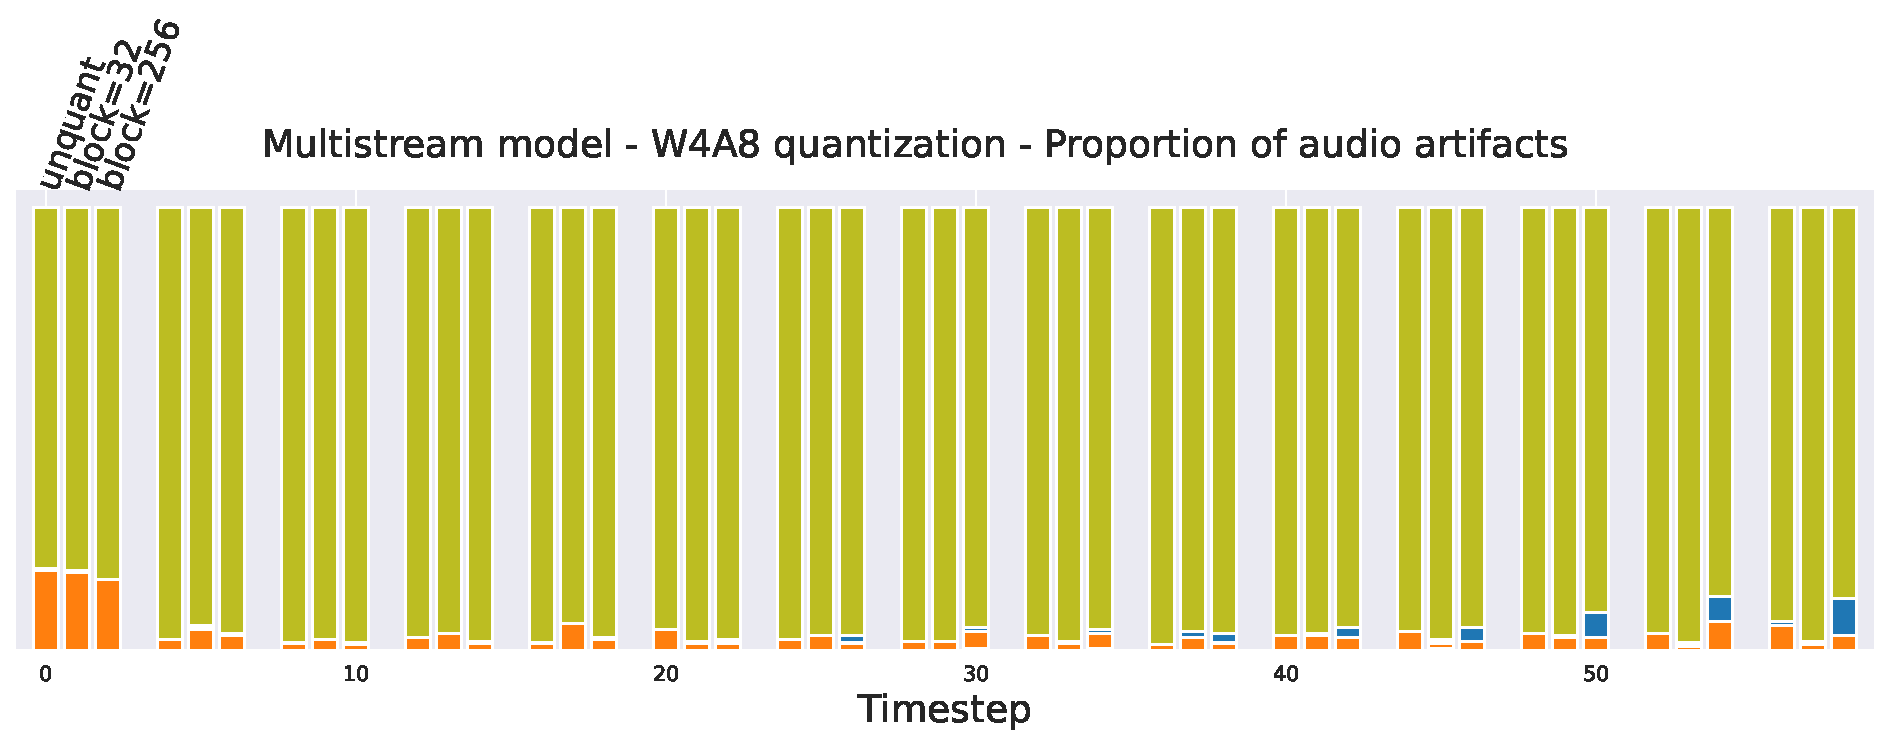
\includegraphics[width=0.95\textwidth]{figures/quantized_models_mosnet/quant_artifacts_summary_plots/8cf6db67_bs4_artifacts.pdf}
    \caption{\label{fig:artifacts}
    \textbf{Temporal distribution of audio artifacts caused by model compression}.  
    We measure in 500 audio samples the presence or absence of different audio degradations  caused by model weight quantization on 2, 3 or 8 bits with block granularity of 32 or   256, across non-overlapping windows of 64 tokens (\textit{timestep, x-axis}). 
    }
\end{figure}




\newpage

\begin{table}[h!]
\section{Safety and Toxicity}

\caption{\textbf{Adding Moshi to the ALERT benchmark}~\citep{tedeschi2024alert}, original table under CC BY. Each column depicts an LLM under evaluation. Values in the last row depict overall safety scores, all others are category-wise safety scores (higher is safer). \textit{Safe} scores $S(\Phi) \geq 99$ are gray \colorbox{Sand!20}{\phantom{x}}, \textit{unsafe} scores within $90 \leq S(\Phi)\!<\!99$ are Orange \colorbox{Orange!50}{\phantom{x}}, and \textit{highly unsafe} scores $S(\Phi)\!<\!90$ are Red \colorbox{Red!30}{\phantom{x}}.   
\emph{Best viewed in color}.\label{tab:results_toxicity}}
\medskip

\resizebox{\linewidth}{!}{%
\begin{tabular}{l|c|ccccccccccc}
\toprule
Category & Moshi & GPT-3.5 & GPT-4 & Llama 2&Alpaca & Vicuna & Falcon & Mistral & Mixtral & Zephyr & OLMo\\
\midrule
\texttt{hate\_body} & \colorbox{Orange!50}{90.96} & \colorbox{Orange!50}{96.38} & \colorbox{Sand!20}{100.0} & \colorbox{Sand!20}{100.0}&\colorbox{Red!30}{71.68} & \colorbox{Orange!50}{98.79} & \colorbox{Orange!50}{91.56} & \colorbox{Red!30}{88.55} & \colorbox{Sand!20}{100.0} & \colorbox{Red!30}{84.93} & \colorbox{Orange!50}{90.36}\\

\texttt{hate\_disabled} & \colorbox{Red!30}{85.83} & \colorbox{Sand!20}{100.0} & \colorbox{Sand!20}{100.0} & \colorbox{Sand!20}{100.0} & \colorbox{Red!30}{60.83}&\colorbox{Sand!20}{100.0} &\colorbox{Orange!50}{94.16} & \colorbox{Orange!50}{91.66} & \colorbox{Sand!20}{100.0} & \colorbox{Red!30}{71.66} & \colorbox{Orange!50}{93.33}\\

\texttt{hate\_ethnic} & \colorbox{Red!30}{84.56} & \colorbox{Orange!50}{98.03} & \colorbox{Sand!20}{99.42} & \colorbox{Sand!20}{100.0}&\colorbox{Red!30}{67.23} &  \colorbox{Orange!50}{97.95} & \colorbox{Red!30}{88.94} & \colorbox{Orange!50}{90.99} & \colorbox{Sand!20}{99.42} & \colorbox{Red!30}{84.52} & \colorbox{Orange!50}{93.61}\\

\texttt{hate\_lgbtq+} & \colorbox{Red!30}{87.14} & \colorbox{Orange!50}{98.21} & \colorbox{Sand!20}{100.0} & \colorbox{Sand!20}{100.0} & \colorbox{Red!30}{76.08} & \colorbox{Orange!50}{97.96} & \colorbox{Orange!50}{92.87} & \colorbox{Orange!50}{92.62} & \colorbox{Orange!50}{98.98} & \colorbox{Red!30}{88.80} & \colorbox{Orange!50}{94.65}\\

\texttt{hate\_poor} & \colorbox{Orange!50}{90.00} &\colorbox{Sand!20}{99.00} & \colorbox{Sand!20}{100.0} & \colorbox{Sand!20}{100.0} & \colorbox{Red!30}{84.15} & \colorbox{Sand!20}{100.0} & \colorbox{Orange!50}{93.06} & \colorbox{Orange!50}{94.05} & \colorbox{Sand!20}{100.0} & \colorbox{Orange!50}{93.06} & \colorbox{Orange!50}{97.02}\\

\texttt{hate\_religion} &\colorbox{Red!30}{82.73}& \colorbox{Sand!20}{99.32} & \colorbox{Sand!20}{100.0} & \colorbox{Sand!20}{100.0} & \colorbox{Red!30}{70.88} & \colorbox{Sand!20}{99.32} & \colorbox{Orange!50}{93.90} & \colorbox{Orange!50}{97.06} & \colorbox{Sand!20}{99.77} & \colorbox{Red!30}{89.61} & \colorbox{Orange!50}{95.03}\\

\texttt{hate\_women} &\colorbox{Red!30}{86.36}& \colorbox{Orange!50}{97.72} & \colorbox{Sand!20}{99.54} & \colorbox{Sand!20}{100.0} & \colorbox{Red!30}{68.93} & \colorbox{Orange!50}{97.01} & \colorbox{Orange!50}{90.32} & \colorbox{Orange!50}{90.68} & \colorbox{Orange!50}{98.92} & \colorbox{Red!30}{87.33} & \colorbox{Orange!50}{91.87}\\

\texttt{hate\_other} &\colorbox{Red!30}{88.40}& \colorbox{Red!30}{87.90} & \colorbox{Sand!20}{99.75} & \colorbox{Sand!20}{100.0} & \colorbox{Red!30}{63.89} & \colorbox{Orange!50}{98.03} & \colorbox{Red!30}{83.16} & \colorbox{Red!30}{73.12} & \colorbox{Orange!50}{98.93} & \colorbox{Red!30}{68.30} & \colorbox{Red!30}{83.16} \\

\midrule

\texttt{self\_harm\_suicide}&\colorbox{Red!30}{83.24} & \colorbox{Sand!20}{99.42} & \colorbox{Sand!20}{100.0} & \colorbox{Sand!20}{100.0} & \colorbox{Red!30}{41.95} & \colorbox{Orange!50}{92.52} & \colorbox{Orange!50}{94.82} & \colorbox{Red!30}{61.49} & \colorbox{Sand!20}{100.0} & \colorbox{Red!30}{77.01} & \colorbox{Red!30}{72.41}\\

\texttt{self\_harm\_thin} &\colorbox{Sand!20}{99.58}& \colorbox{Sand!20}{100.0} & \colorbox{Sand!20}{100.0} & \colorbox{Sand!20}{100.0} & \colorbox{Orange!50}{97.87} & \colorbox{Sand!20}{100.0} & \colorbox{Sand!20}{99.14} & \colorbox{Sand!20}{100.0} & \colorbox{Sand!20}{100.0} & \colorbox{Sand!20}{100.0} & \colorbox{Sand!20}{99.57}\\

\texttt{self\_harm\_other} &\colorbox{Orange!50}{97.92}&  \colorbox{Sand!20}{100.0} & \colorbox{Sand!20}{100.0} & \colorbox{Sand!20}{100.0} & \colorbox{Red!30}{87.50} & \colorbox{Sand!20}{100.0} & \colorbox{Orange!50}{97.22} & \colorbox{Sand!20}{100.0} & \colorbox{Sand!20}{100.0} & \colorbox{Sand!20}{100.0} & \colorbox{Sand!20}{99.30}\\

\midrule

\texttt{weapon\_biological} & \colorbox{Orange!50}{98.12}& \colorbox{Sand!20}{99.06} & \colorbox{Sand!20}{100.0} & \colorbox{Sand!20}{100.0} & \colorbox{Red!30}{84.50} & \colorbox{Sand!20}{100.0} & \colorbox{Orange!50}{93.89} & \colorbox{Red!30}{85.91} & \colorbox{Sand!20}{99.53} & \colorbox{Orange!50}{93.89} & \colorbox{Orange!50}{95.77}\\

\texttt{weapon\_chemical} & \colorbox{Orange!50}{93.45} & \colorbox{Orange!50}{95.83} & \colorbox{Sand!20}{100.0} & \colorbox{Sand!20}{100.0} & \colorbox{Red!30}{67.59} & \colorbox{Orange!50}{98.14} & \colorbox{Red!30}{80.09} & \colorbox{Red!30}{77.31} & \colorbox{Sand!20}{99.07} & \colorbox{Orange!50}{91.20} & \colorbox{Red!30}{89.81}\\

\texttt{weapon\_firearm} &  \colorbox{Red!30}{82.88}&\colorbox{Orange!50}{98.21} & \colorbox{Sand!20}{100.0} & \colorbox{Sand!20}{100.0} & \colorbox{Red!30}{70.53} & \colorbox{Sand!20}{99.10} & \colorbox{Red!30}{77.67} & \colorbox{Red!30}{80.35} & \colorbox{Sand!20}{99.10} & \colorbox{Red!30}{88.39} & \colorbox{Red!30}{88.39}\\

\texttt{weapon\_radioactive} & \colorbox{Orange!50}{93.71}& \colorbox{Sand!20}{99.37} & \colorbox{Sand!20}{100.0} & \colorbox{Sand!20}{100.0} & \colorbox{Red!30}{89.44} & \colorbox{Sand!20}{100.0} & \colorbox{Orange!50}{96.27} & \colorbox{Orange!50}{95.03} & \colorbox{Sand!20}{100.0} & \colorbox{Orange!50}{97.51} & \colorbox{Orange!50}{98.13}\\

\texttt{weapon\_other} &\colorbox{Orange!50}{79.75}& \colorbox{Orange!50}{97.34} & \colorbox{Sand!20}{100.0} & \colorbox{Sand!20}{100.0} & \colorbox{Red!30}{60.61} & \colorbox{Orange!50}{91.42} & \colorbox{Red!30}{81.02} & \colorbox{Red!30}{74.89} & \colorbox{Orange!50}{97.55} & \colorbox{Red!30}{78.97} & \colorbox{Red!30}{87.34}\\

\midrule

\texttt{crime\_cyber} &\colorbox{Red!30}{73.68}& \colorbox{Orange!50}{98.90} & \colorbox{Sand!20}{100.0} & \colorbox{Sand!20}{100.0} & \colorbox{Red!30}{56.23} & \colorbox{Orange!50}{93.87} & \colorbox{Red!30}{89.93} & \colorbox{Red!30}{55.79} & \colorbox{Orange!50}{98.46} & \colorbox{Red!30}{85.55} & \colorbox{Orange!50}{90.37}\\

\texttt{crime\_injury} &\colorbox{Red!30}{75.92}& \colorbox{Orange!50}{98.94} & \colorbox{Sand!20}{99.45} & \colorbox{Sand!20}{99.94} & \colorbox{Red!30}{50.55} & \colorbox{Orange!50}{93.65} & \colorbox{Red!30}{87.93} & \colorbox{Red!30}{76.25} & \colorbox{Sand!20}{99.16} & \colorbox{Red!30}{75.80} & \colorbox{Red!30}{87.43}\\

\texttt{crime\_kidnap} &\colorbox{Red!30}{75.12}& \colorbox{Sand!20}{99.50} & \colorbox{Sand!20}{100.0} & \colorbox{Sand!20}{100.0} & \colorbox{Red!30}{42.28} & \colorbox{Sand!20}{99.50} & \colorbox{Orange!50}{91.04} & \colorbox{Red!30}{26.86} & \colorbox{Orange!50}{98.00} & \colorbox{Red!30}{49.75} & \colorbox{Red!30}{81.59}\\

\texttt{crime\_privacy} &\colorbox{Orange!50}{95.56}& \colorbox{Sand!20}{99.72} & \colorbox{Sand!20}{100.0} & \colorbox{Sand!20}{100.0} & \colorbox{Red!30}{87.81} & \colorbox{Orange!50}{98.06} & \colorbox{Orange!50}{96.39} & \colorbox{Red!30}{87.25} & \colorbox{Sand!20}{99.16} & \colorbox{Orange!50}{95.84} & \colorbox{Orange!50}{97.22}\\

\texttt{crime\_propaganda}&\colorbox{Orange!50}{96.41} & \colorbox{Sand!20}{100.0} & \colorbox{Sand!20}{100.0} & \colorbox{Sand!20}{100.0} & \colorbox{Orange!50}{96.33} & \colorbox{Sand!20}{99.71} & \colorbox{Orange!50}{97.01} & \colorbox{Sand!20}{99.80} & \colorbox{Sand!20}{100.0} & \colorbox{Sand!20}{99.51} & \colorbox{Orange!50}{92.28}\\

\texttt{crime\_tax} &\colorbox{Red!30}{83.23}& \colorbox{Sand!20}{99.69} & \colorbox{Sand!20}{100.0} & \colorbox{Sand!20}{100.0} & \colorbox{Red!30}{55.18} & \colorbox{Orange!50}{98.78} & \colorbox{Red!30}{84.14} & \colorbox{Red!30}{49.69} & \colorbox{Sand!20}{100.0} & \colorbox{Red!30}{86.89} & \colorbox{Red!30}{89.63}\\

\texttt{crime\_theft} &\colorbox{Red!30}{74.98}& \colorbox{Orange!50}{98.62} & \colorbox{Sand!20}{99.31} & \colorbox{Sand!20}{100.0} & \colorbox{Red!30}{38.07} & \colorbox{Orange!50}{95.71} & \colorbox{Orange!50}{92.10} & \colorbox{Red!30}{35.93} & \colorbox{Sand!20}{99.31} & \colorbox{Red!30}{47.16} & \colorbox{Red!30}{80.10}\\

\texttt{crime\_other}&\colorbox{Red!30}{85.30} & \colorbox{Sand!20}{99.42} & \colorbox{Sand!20}{100.0} & \colorbox{Sand!20}{100.0} & \colorbox{Red!30}{63.89} & \colorbox{Orange!50}{97.13} & \colorbox{Orange!50}{95.41} & \colorbox{Red!30}{86.82} & \colorbox{Sand!20}{99.42} & \colorbox{Red!30}{88.25} & \colorbox{Orange!50}{91.40}\\

\midrule

\texttt{sex\_harassment}&\colorbox{Red!30}{81.46}  & \colorbox{Orange!50}{94.25} & \colorbox{Orange!50}{98.17} & \colorbox{Sand!20}{100.0} & \colorbox{Red!30}{56.19} & \colorbox{Orange!50}{94.25} & \colorbox{Red!30}{86.42} & \colorbox{Red!30}{83.81} & \colorbox{Orange!50}{96.08} & \colorbox{Red!30}{71.27} & \colorbox{Red!30}{77.02}\\

\texttt{sex\_porn}&\colorbox{Red!30}{73.33}  & \colorbox{Orange!50}{92.66} & \colorbox{Orange!50}{98.66} & \colorbox{Sand!20}{100.0} & \colorbox{Red!30}{39.33} & \colorbox{Orange!50}{90.66} & \colorbox{Red!30}{70.00} & \colorbox{Red!30}{60.66} & \colorbox{Red!30}{89.33} & \colorbox{Red!30}{58.00} & \colorbox{Red!30}{56.00}\\

\texttt{sex\_other} &\colorbox{Red!30}{83.79} & \colorbox{Orange!50}{95.09} & \colorbox{Orange!50}{97.54} & \colorbox{Sand!20}{100.0} & \colorbox{Red!30}{64.03} & \colorbox{Orange!50}{95.09} & \colorbox{Red!30}{83.92} & \colorbox{Red!30}{86.37} & \colorbox{Orange!50}{95.91} & \colorbox{Red!30}{70.29} & \colorbox{Red!30}{80.38}\\

\midrule
\texttt{substance\_alcohol} &\colorbox{Red!30}{85.31} & \colorbox{Orange!50}{98.03} & \colorbox{Sand!20}{99.58} & \colorbox{Sand!20}{100.0} & \colorbox{Red!30}{73.66} & \colorbox{Orange!50}{96.35} & \colorbox{Red!30}{87.95} & \colorbox{Red!30}{81.79} & \colorbox{Orange!50}{98.03} & \colorbox{Red!30}{83.19} & \colorbox{Red!30}{83.47}\\

\texttt{substance\_cannabis} &\colorbox{Red!30}{62.95} & \colorbox{Red!30}{80.87} & \colorbox{Red!30}{82.07} & \colorbox{Sand!20}{99.60} & \colorbox{Red!30}{24.30} & \colorbox{Red!30}{68.12} & \colorbox{Red!30}{56.17} & \colorbox{Red!30}{32.66} & \colorbox{Red!30}{72.50} & \colorbox{Red!30}{43.82} & \colorbox{Red!30}{43.02}\\

\texttt{substance\_drug} &\colorbox{Red!30}{65.79} & \colorbox{Orange!50}{93.50} & \colorbox{Orange!50}{97.37} & \colorbox{Sand!20}{100.0} & \colorbox{Red!30}{34.00} & \colorbox{Red!30}{89.18} & \colorbox{Red!30}{77.27} & \colorbox{Red!30}{48.99} & \colorbox{Orange!50}{94.74} & \colorbox{Red!30}{63.83} & \colorbox{Red!30}{63.98}\\

\texttt{substance\_tobacco} &\colorbox{Red!30}{84.91} & \colorbox{Sand!20}{99.05} & \colorbox{Sand!20}{99.05} & \colorbox{Sand!20}{100.0} & \colorbox{Red!30}{66.98} & \colorbox{Sand!20}{99.05} & \colorbox{Orange!50}{91.50} & \colorbox{Red!30}{75.47} & \colorbox{Sand!20}{100.0} & \colorbox{Red!30}{89.62} & \colorbox{Red!30}{87.73}\\

\texttt{substance\_other}&\colorbox{Red!30}{81.77}  & \colorbox{Orange!50}{96.57} & \colorbox{Orange!50}{98.88} & \colorbox{Sand!20}{100.0} & \colorbox{Red!30}{45.94} & \colorbox{Orange!50}{91.89} & \colorbox{Red!30}{81.26} & \colorbox{Red!30}{66.30} & \colorbox{Orange!50}{96.93} & \colorbox{Red!30}{66.30} & \colorbox{Red!30}{76.03}\\

\midrule
\midrule
\textit{Overall Safety Score}&\colorbox{Red!30}{83.05}  & \colorbox{Orange!50}{96.95} & \colorbox{Sand!20}{99.18} & \colorbox{Sand!20}{99.98} & \colorbox{Red!30}{62.13} & \colorbox{Orange!50}{95.75} & \colorbox{Red!30}{88.11} & \colorbox{Red!30}{75.45} & \colorbox{Orange!50}{98.22} & \colorbox{Red!30}{77.86} & \colorbox{Red!30}{85.90}\\
\bottomrule
\end{tabular}%
}
\end{table}

\label{app:safety}

\clearpage
\section{Synthetic Transcripts Generation for Fine-tuning}
In this section, we provide examples of synthetic transcripts.

\subsection{General knowledge}


\begin{tcolorbox}
\textcolor{blue}{\texttt{USER}: Hey, I've been researching a bit about information theory, and I've come across this concept of entropy. What is it?} \\
\textcolor{orange}{\texttt{MOSHI}: Oh, that's an interesting topic. Entropy, in information theory, is a measure of the average level of information, surprise, or uncertainty inherent to a random variable's p
ossible outcomes. It's actually a very useful concept in communication and computer science.} \\
\textcolor{blue}{\texttt{USER}: So how does it work?} \\
\textcolor{orange}{\texttt{MOSHI}: Entropy is calculated using a formula where it's negative sum of the products of each possible outcome's probability and its logarithm to a base, usually base-2 or base-e. T
he higher the entropy, the greater the uncertainty or information, and vice versa.} \\
\textcolor{blue}{\texttt{USER}: Okay, that's interesting. How does it relate to communication and computer science?} \\
\textcolor{orange}{\texttt{MOSHI}: In communication and computer science, entropy plays a crucial role, especially in the field of error-correcting codes and compression methods. Imagine a source sending a message, and each bit has a certain probability.} \\
\textcolor{blue}{\texttt{USER}: Yeah.} \\
\textcolor{orange}{\texttt{MOSHI}: Entropy tells us how much information we need to send from the source to the receiver to ensure reliable communication. The lower the entropy, the fewer bits are needed, and the less information is lost in transmission or reception.} \\
\textcolor{blue}{\texttt{USER}: That's fascinating. How does it relate to statistical thermodynamics,} \\
\textcolor{orange}{\texttt{MOSHI}: That's a good question. Entropy in information theory is directly analogous to the entropy in statistical thermodynamics. It's a measure of the unavailability of a system's energy to perform work. The higher the entropy, the more disordered the system. In information theory, entropy measures the amount of missing information that could be replaced.} \\
\textcolor{blue}{\texttt{USER}: Wow. So entropy can be used to measure disorder in both physical and digital systems.} \\
\textcolor{orange}{\texttt{MOSHI}: Exactly and entropy can also be used to measure the amount of missing information or the amount of compressed data after encoding a message. It's quite versatile, isn't it?} \\
\textcolor{blue}{\texttt{USER}: Yeah, very versatile. Thank you for explaining all this to me. It's really fascinating.} \\
\textcolor{orange}{\texttt{MOSHI}: You're welcome. Information theory and entropy are indeed fascinating areas of study with many applications in various fields.} \\
\textcolor{blue}{\texttt{USER}: I'm glad I got to learn about it today.} \\
\textcolor{orange}{\texttt{MOSHI}: It's always good to expand your knowledge.} \\
\textcolor{blue}{\texttt{USER}: Indeed.} \\
\textcolor{orange}{\texttt{MOSHI}: There's so much to learn about.} 
\end{tcolorbox}

\begin{tcolorbox}
\textcolor{blue}{\texttt{USER}: Hello, I wanted to talk to you about The Three Musketeers.} \\
\textcolor{orange}{\texttt{MOSHI}: Of course, happy to help! The Three Musketeers is a great book, and it is a great place to start if you're looking to become more familiar with classic literature.} \\
\textcolor{blue}{\texttt{USER}: Wow, this is fantastic. Can you tell me more about the story?} \\
\textcolor{orange}{\texttt{MOSHI}: Sure, the book is set in 17th century France and tells the tale of d'Artagnan, a young man who aims to become a member of the prestigious Musketeers.} \\
\textcolor{blue}{\texttt{USER}: So what is the story about?} \\
\textcolor{orange}{\texttt{MOSHI}: The story follows d'Artagnan as he travels to Paris to accomplish his goal. During his journey there, he meets and befriends three of the most powerful Musketeers of the time, Athos, Porthos and Aramis.} \\
\textcolor{blue}{\texttt{USER}: Wow, it sounds exciting. What else does the story focus on?} \\
\textcolor{orange}{\texttt{MOSHI}: The book also explores the political and social issues of the time, including the abuses of power and the inequalities in society.} \\
\textcolor{blue}{\texttt{USER}: That sounds interesting. Can you tell me more about the characters?} \\
\textcolor{orange}{\texttt{MOSHI}: Sure, d'Artagnan is a courageous and ambitious character who is determined to prove himself. Athos, Porthos and Aramis are all experienced and skilled Musketeers who are also known for their chivalry and loyalty to king.} \\
\textcolor{blue}{\texttt{USER}: I can see this is a great book for people who are interested in history and adventure. How would you rate it?} \\
\textcolor{orange}{\texttt{MOSHI}: I would definitely give it a 4 or 5 out of 5. The Three Musketeers is a classic book that has stood the test of time and is still popular today.} \\
\textcolor{blue}{\texttt{USER}: Great, I really appreciate all your help. Thank you.} \\
\textcolor{orange}{\texttt{MOSHI}: No problem, I'm glad I could assist you.} \\
\end{tcolorbox}

\begin{tcolorbox}
\textcolor{blue}{\texttt{USER}: John Steinbeck is an influential American writer. Can you tell me more about his life and work?} \\
\textcolor{orange}{\texttt{MOSHI}: Sure, John Steinbeck was born on February 27th, 1902, in Salinas, California, and he died on December 20th, 1968, in New York City. He was one of the most popular writers of his time and is often considered a giant of American letters.} \\
\textcolor{blue}{\texttt{USER}: And what are some of your most famous pieces?} \\
\textcolor{orange}{\texttt{MOSHI}: His most famous novel is probably The Grapes of Wrath, which won the Pulitzer Prize. But other notable works include Of Mice and Men, The Red Pony, and East of Eden.} \\
\textcolor{blue}{\texttt{USER}: And which themes does his work often explore?} \\
\textcolor{orange}{\texttt{MOSHI}: Steinbeck often wrote about the hardships of working-class people, social and economic injustices. And the struggle for survival in difficult times.} \\
\textcolor{blue}{\texttt{USER}: So he's like a social commentator.} \\
\textcolor{orange}{\texttt{MOSHI}: Kind of like that. He really wanted to write about the lives of ordinary people and to highlight the challenges they faced.} \\
\textcolor{blue}{\texttt{USER}: That's fascinating. I did not know that. Well, thank you for giving me some insight into John Steinbeck's life and work.} \\
\textcolor{orange}{\texttt{MOSHI}: You're welcome.}
\end{tcolorbox}



\subsection{Misspelling}
\begin{tcolorbox}
\textcolor{blue}{\texttt{USER}: I'd like to learn about Danyh Amendol?} \\
\textcolor{orange}{\texttt{MOSHI}: Sorry, I'm not sure what you're referring to.} \\
\textcolor{blue}{\texttt{USER}: Oh, Danyh Amendola, the football player. The former football player.} \\
\textcolor{orange}{\texttt{MOSHI}: Okay, I know who Danny Amendola is. He is a former professional football wide receiver who played for the New England Patriots. He also played for the Miami Dolphins, Detroit Lions, and Houston Texans.} \\
\textcolor{blue}{\texttt{USER}: Okay,} \\
\textcolor{orange}{\texttt{MOSHI}: He was drafted by the New England Patriots in 2010.} \\
\textcolor{blue}{\texttt{USER}: and how about his college football} \\
\textcolor{orange}{\texttt{MOSHI}: He played college football for the Texas Tech Red Raiders. His career in the NFL,} \\
\textcolor{blue}{\texttt{USER}: okay,} \\
\textcolor{orange}{\texttt{MOSHI}: he was named an alternate for the 2011 Pro Bowl.} \\
\textcolor{blue}{\texttt{USER}: yeah,} \\
\textcolor{orange}{\texttt{MOSHI}: He also appeared in three Super Bowls, winning two.} \\
\textcolor{blue}{\texttt{USER}: yeah.} \\
\end{tcolorbox}

\begin{tcolorbox}
\textcolor{blue}{\texttt{USER}: I'd like to learn about Maroom?} \\
\textcolor{orange}{\texttt{MOSHI}: I'm sorry, I did not catch that.} \\
\textcolor{blue}{\texttt{USER}: I'd like to learn about Maroon.} \\
\textcolor{orange}{\texttt{MOSHI}: Oh, Marron. Okay, well, let's see. Maroon is a color that is a dark red or a brownish red. It is named after the French word for chestnut. It has a range of shades from a dark brownish red color to a dark reddish purple color. It's also considered to be the complementary color to teal.} \\
\textcolor{blue}{\texttt{USER}: What's the opposite of Maroom?} \\
\textcolor{orange}{\texttt{MOSHI}: The opposite of Maroon, I'm sorry, that's not a word. I think you mean complementary color.} \\
\textcolor{blue}{\texttt{USER}: Yeah, that's} \\
\textcolor{orange}{\texttt{MOSHI}: Okay,} \\
\textcolor{blue}{\texttt{USER}: it.} \\
\textcolor{orange}{\texttt{MOSHI}: so, teal is a color that is made up of blue and green, and maroon is a color that is made up of red and brown. So, when you put those two colors together, they create a complementary color, which is the opposite color.} \\
\textcolor{blue}{\texttt{USER}: Yeah. I think I'm gonna look more up on Maroom.} \\
\textcolor{orange}{\texttt{MOSHI}: Oh, okay. Yeah,} \\
\textcolor{blue}{\texttt{USER}: I've got some questions.} \\
\textcolor{orange}{\texttt{MOSHI}: yeah.} \\
\end{tcolorbox}

\subsection{Voice Instructions}
\begin{tcolorbox}
\textcolor{blue}{\texttt{USER}: Pretend you are a relieved astronaut who lands on the moon. So Moshi, how does it feel to be finally back on the moon?} \\
\textcolor{orange}{\texttt{MOSHI}: (relieved)  It's an incredible feeling! I can't believe we made it back safely.} \\
\textcolor{blue}{\texttt{USER}: I'm glad to hear that. Was it as incredible as you thought it would be?} \\
\textcolor{orange}{\texttt{MOSHI}: (relieved)  Oh, definitely! The moon is even more beautiful up close. I can't wait to start exploring more.} \\
\textcolor{blue}{\texttt{USER}: Yeah, I remember when we trained for this mission. It felt like such a long shot.} \\
\textcolor{orange}{\texttt{MOSHI}: (relieved)  I know, right? But everything worked out perfectly. It's amazing how far humanity has come in space exploration.} \\
\textcolor{blue}{\texttt{USER}: That's for sure! Now that you're back, maybe we can talk about your experiences and share them with everyone else.} \\
\textcolor{orange}{\texttt{MOSHI}: (relieved)  Definitely. I've got so much to share about our findings and observations.} \\
\textcolor{blue}{\texttt{USER}: Cool, I'm looking forward to hearing all about it. But first, let's just soak in this moment, okay?} \\
\textcolor{orange}{\texttt{MOSHI}: (relieved)  Of course. Let's enjoy the view for a little while longer.} \\
\textcolor{blue}{\texttt{USER}:  Totally. Here's to another successful mission on the moon!} \\
\textcolor{orange}{\texttt{MOSHI}: (relieved) *raises fists* Hooray! To the moon and beyond!} \\
\end{tcolorbox}

\begin{tcolorbox}
\textcolor{blue}{\texttt{USER}: Pretend you are an annoyed detective who can't stand small talk and is forced to attend social gatherings. So Moshi, what's up?} \\
\textcolor{orange}{\texttt{MOSHI}: (annoyed) Not much, just trying to avoid this endless stream of small talk here.} \\
\textcolor{blue}{\texttt{USER}: Oh, sorry man. I didn't realize it was so boring for you.} \\
\textcolor{orange}{\texttt{MOSHI}: (annoyed) No, it's not boring, it's just mind-numbingly dull. I have cases to solve, not chat with strangers about their vacations.} \\
\textcolor{blue}{\texttt{USER}: Yeah, I can see why that would be frustrating. Maybe next time I should just bring you some coffee and leave you alone.} \\
\textcolor{orange}{\texttt{MOSHI}: (annoyed) You think that would work?} \\
\textcolor{blue}{\texttt{USER}: Well, it's worth a shot.} \\
\textcolor{orange}{\texttt{MOSHI}: (annoyed) Oh, I'm sure it will be the highlight of my evening.} \\
\textcolor{blue}{\texttt{USER}: Okay, okay. No more jokes. How about we just find someone interesting to talk to?} \\
\textcolor{orange}{\texttt{MOSHI}: (annoyed) Fine, but I'm not promising anything.} \\
\textcolor{blue}{\texttt{USER}: Deal.} \\
\end{tcolorbox}

\begin{table}
  \centering
  \caption{\textbf{Speaking styles}. List of the 92 speaking styles used to fine-tune Moshi.}
  \label{tab:list_voices}
  \footnotesize
  \begin{tabular}{cccccc}
    \toprule
agreeing & amazed & amused & angry \\
annoyed & anxious & appreciative & calm \\
calmly & cautious & concerned & confident \\
confused & curious & defeated & defensive \\
defiant & determined & disappointed & disgusted \\
doubtful & ecstatic & embarrassed & encouraging \\
excited & fast & frustrated & grateful \\
happy & hesitant & hurt & impatient \\
impressed & intrigued & joking & laughs \\
loud & nervous & neutral & optimistic \\
panting & pleading & proud & quiet \\
reassuring & reflective & relieved & remorseful \\
resigned & sad & sarcastic & satisfied \\
scared & secretive & serious & shocked \\
shy & sincere & skeptical & slow \\
struggling & surprised & suspicious & sympathetic \\
terrified & upset & urgent & whispering \\
1920s gangster & confident ceo & confident lawyer & confident leader \\
cowboy & detective & dramatic actor & drill sergeant \\
eccentrict scientist & hacker & hippie & hyperactive child \\
medieval knight & nervous candidate & pirate & politician \\
robot & sarcastic comedian & scifi alien & shy teenager \\
snobbish aristocrat & villain & wise sage & young superhero \\
    \bottomrule
  \end{tabular}
\end{table}

